% ---------------------------------------------------- %
%                CONFIGURATION                         %
% ---------------------------------------------------- %

\documentclass[twoside]{article}

\usepackage{lipsum} % Package to generate dummy text throughout this template
\usepackage{amsmath}
\usepackage[sc]{mathpazo} % Use the Palatino font
\usepackage[T1]{fontenc} % Use 8-bit encoding that has 256 glyphs
\linespread{1.05} % Line spacing - Palatino needs more space between lines
\usepackage{microtype} % Slightly tweak font spacing for aesthetics
\usepackage[hmarginratio=1:1,top=32mm,columnsep=20pt,left=0.8in,right=0.8in]{geometry} % Document margins
\usepackage{multicol} % Used for the two-column layout of the document
\usepackage[hang, small,labelfont=bf,up,textfont=it,up]{caption} % Custom captions under/above floats in tables or figures
\usepackage{booktabs} % Horizontal rules in tables
\usepackage{float} % Required for tables and figures in the multi-column environment - they need to be placed in specific locations with the [H] (e.g. \begin{table}[H])
\usepackage{hyperref} % For hyperlinks in the PDF

\usepackage{lettrine} % The lettrine is the first enlarged letter at the beginning of the text
\usepackage{paralist} % Used for the compactitem environment which makes bullet points with less space between them

\usepackage{abstract} % Allows abstract customization
\renewcommand{\abstractnamefont}{\normalfont\bfseries} % Set the "Abstract" text to bold
\renewcommand{\abstracttextfont}{\normalfont\small\itshape} % Set the abstract itself to small italic text

\usepackage{titlesec} % Allows customization of titles
\renewcommand\thesection{\Roman{section}} % Roman numerals for the sections
\renewcommand\thesubsection{\Roman{subsection}} % Roman numerals for subsections
\titleformat{\section}[block]{\large\scshape\centering}{\thesection.}{1em}{} % Change the look of the section titles
\titleformat{\subsection}[block]{\large}{\thesubsection.}{1em}{} % Change the look of the section titles

\usepackage{fancyhdr} % Headers and footers
\pagestyle{fancy} % All pages have headers and footers
\fancyhead{} % Blank out the default header
\fancyfoot{} % Blank out the default footer
\fancyhead[C]{Efficient Coding Hypothesis and an Introduction to Information Theory $\star$ September 2014} % Custom header text
\fancyfoot[RO,LE]{\thepage} % Custom footer text

\usepackage{graphicx}


% ---------------------------------------------------- %
%                CONFIGURATION                         %
% ---------------------------------------------------- %



% ---------------------------------------------------- %
%                   	TITLE                          %
% ---------------------------------------------------- %

\title{\vspace{-15mm}\fontsize{24pt}{10pt}\selectfont\textbf{Efficient Coding Hypothesis and an introduction to information Theory}} % Article title
\author{Lay Kuan Loh \& Mihovil Bartulovic}
\date{\today}

% ---------------------------------------------------- %
%                   	TITLE                          %
% ---------------------------------------------------- %



\begin{document}

\maketitle % Insert title

\thispagestyle{fancy} % All pages have headers and footers




% ---------------------------------------------------- %
%                   	ABSTRACT                       %
% ---------------------------------------------------- %

\begin{abstract}

\noindent The Efficient Coding Hypothesis, proposed by Barlow 1961, suggests that sensory relays recode sensory messages, so that their redundancy is reduced, but little information is lost. Coding to reduce redundancy not just eliminates wasteful neural activity, but also organizes sensory information such than an internal model of the environment causing the pst sensory inputs ins built up, while the current sensory situation is represented in a way that simplified the task of the parts of the nervours ssystem responsible for learning and conditioning. To investigate animals' sensory mechanisms, Barlow 1961 suggests that one examine the ways in which animals use their senses, as these ways are likely reflected in the design of the sense organs and their nervous pathways.

\end{abstract}

% ---------------------------------------------------- %
%                   	ABSTRACT                       %
% ---------------------------------------------------- %








% ---------------------------------------------------- %
%                   	INTRODUCTION                   %
% ---------------------------------------------------- %

\begin{multicols}{2} % Two-column layout throughout the main article text

\section{Introduction}

\lettrine[nindent=0em,lines=3]{L} orem ipsum dolor sit amet, consectetur adipiscing elit.
\lipsum[2-3] 

% ---------------------------------------------------- %
%                   	INTRODUCTION                   %
% ---------------------------------------------------- %



% ---------------------------------------------------- %
%                      BARLOW 1961                     %
% ---------------------------------------------------- %

\section{Possible Principles Underlying the Transformations of Sensory Messages}



% ---------------------------------------------------- %
%                      BARLOW 1961                     %
% ---------------------------------------------------- %



% ---------------------------------------------------- %
%                	NIRENBERG 2001                     %
% ---------------------------------------------------- %

\section{Retinal ganglion cells act largely as independent encoders}

\footnotesize
Correlated firing among neurons is widespread in the visual system, but its importance for encoding visual information is unclear. To study this, Nirenberg et. al., 2001 presented the retina with natural stimuli and computed the responses of the output cells, the ganglion cells. They used information theoretic techniques to measure the amount of information about the stimuli that can be obtained from the cells under correlated firing and non-correlated firing. They found that more than 90\% of the information about the stimuli can be obtained from the cells with uncorrelated firing, suggesting that ganglion cells act largely independently to encode information, simplifying the problem of decoding their activity. 

\normalsize
Nirenberg et. al., 2001 stimulated pairs of isolated mouse retina using natural movies. The stimuli were each 7 seconds long and repeated 300 times, and the ganglion cell responses were recorded. Data used had to be clean of contaminating spikes from other cells, and that both responses had to have average firing rates. 

To find the degree of correlated activity for each pair, the excess correlated fraction (ECF) was found. ECF is the fraction of correlated spikes produced by the pair above chance, taking into account correlations induced by the stimulus. The ECFs ranged from -1\% to 34\%. 

To measure the amount of information the pairs of ganglion cells carried about the stimuli when their correlations were taken into account, information theoretic techniques were used. Each movie was treated as a series of segments of fixed temporal length, with each segment regarded as a separate stimulus. The movie was presented several hundred times to generate a large set of responses (spike trains) to each segment. This allowed the authors to estimate the probability of getting a particular pair of responses given a particular movie segment - that is, to estimate $\mathbb{P}(r_1,r_2|s)$, where $r_1$ was the response of cell 1, $r_2$ was the response of cell 2 and $s$ was the movie segment. Given these conditional probabilities, the amount of information $I$ between the responses and the stimulus segments was found using the expression:


\begin{align}\label{eq:info-theory}
	I 
		&= -\sum_{r_1,r_2}\mathbb{P}(r_1,r_2)\log_2\mathbb{P}(r_1,r_2) \\
  		&+ \sum_s\mathbb{P}(s) \sum_{r_1,r_2}\mathbb{P}(r_1,r_2|s)\log_2\mathbb{P}(r_1,r_2|s)
\end{align}


where $\mathbb{P}(r_1,r_2)$ is found by taking $\mathbb{P}(r_1,r_2) = \sum_s \mathbb{P}(r_1,r_2|s)\mathbb{P}(s)$, and $\mathbb{P}(s)$ is the probability that a given stimulus segment $s$ occured. 

To examine how important correlation is in encoding visual information, the amount of information that would be lost if the correlations in the responses of the pair of ganglion cells were ignored was examined. To ignore the correlations, the conditional probability distributions of the two responses, $\mathbb{P}(r_1,r_2|s)$, as the product of their individual probability distributions, $\mathbb{P}(r_1|s)$ and $\mathbb{P}(r_2|s)$. $\mathbb{P}(r_1|s)\mathbb{P}(r_1|s)$ to estimate the probability of a stimulus given a response. As $\mathbb{P}(r_1|s)\mathbb{P}(r_1|s)$ is not quite the true distribution, using it should lead to a loss of information. 

Therefore, the amount of independent information is given by

\begin{align}
	I_{IND} 
		&= -\sum_{r_1,r_2}\mathbb{P}(r_1,r_2|s)\log_2\mathbb{P}(r_1|s)\mathbb{P}(r_2|s) \\
		&+ \sum_s\mathbb{P}(s) \sum_{r_1,r_2}\mathbb{P}(r_1,r_2|s)\log_2\mathbb{P}(r_1|s)\mathbb{P}(r_2|s) 
\end{align}

The amount of information in bits lost, $\Delta I$, is given by 
\begin{align}
	\Delta I 
		&= I - I_{IND} \\
		&= \sum_s\mathbb{P}(s) \sum_{r_1,r_2}\mathbb{P}(r_1,r_2|s) \log_2 \frac{\mathbb{P}(r_1,r_2|s)}{\mathbb{P}(r_1|s)\mathbb{P}(r_2|s)} \\
		&- \sum_{r_1,r_2}\mathbb{P}(r_1,r_2) \log_2 \frac{\mathbb{P}(r_1,r_2)}{\sum_s \mathbb{P}(r_1|s)\mathbb{P}(r_2|s) \mathbb{P}(s)} 
\end{align}

$\Delta I$ is very small, as most pairs lost less than 10\% of information. If there were pairs of ganglion cells with higher degrees of correlation than the maximum 34\% observed, more information loss could have occured. This finding means that strategies used to decode ganglion cell activity, which treat the cells as independent encoders are reasonable, as they can capture more than 90\% of the information the cells carry. Furthermore, the activity of any given ganglion cell can be evaluated separately from other cells, without accounting for other cells in the population. This allows the problem of decoding population activity to be significanly simplified, as much less data is needed to analyze the uncorrelated case as opposed to the correlated case. 

Several concerns with the study are that capturing more than 90\% in ganglion cell activity may not be enough to fully understand its activity. Also, perhaps correlation should not be ignored for the activity of a larger population of cells than just pairs of cells studied here. 

% ---------------------------------------------------- %
%                	NIRENBERG 2001                     %
% ---------------------------------------------------- %





% ---------------------------------------------------- %
%                    LAUGHLIN 1981                     %
% ---------------------------------------------------- %

\section{A Simple Coding Procedure Enhances a Neuron's Information Capacity}

Neurons carry and process information. Large monopolar cells (LMC's) are first order interneurons of the insect compound eye, with graded responses driven by small groups of receptors with the same field of view. The compressive intensity-response function of the receptors, combined with lateral and self-inhibition, adjusts the LMC sensitivity to the background intensity so that their responses code contrast fluctuations rather than absolute intensity. Laughlin 1981 shows that the interneuron's contrast-response function matches the range of contrasts encountered in natural scenes, which increases the efficiency with which information is encoded. 

A fundamental limitation on neural coding is the restricted range of responses with which a neuron can represent the states of its inputs. The LMC cell's response range is limited by reversal potentials. If the sensitivities of a neuron are too high, inputs would often saturate the response, and informatio will be lost through clipping. If the sensitivities are too low, large parts of the response range are underutilized because they correspond to exceptionally large ranges of input. Information theory suggests that the most efficient way to apportion the neuron's limited response range is to encode inputs so that all response levels are used with equal frequency. Thus, information carried by the responses can be maximised because the information channel achieves its maximum entropy. 

The simplest case is when a neuron represents a single input parameter with a single output parameter. For this case, the optimum can be reaches when the input-output function corresponds to the cumulative probability function for the different input levels. 

\begin{figure}[H]
	\caption{This is a caption}
	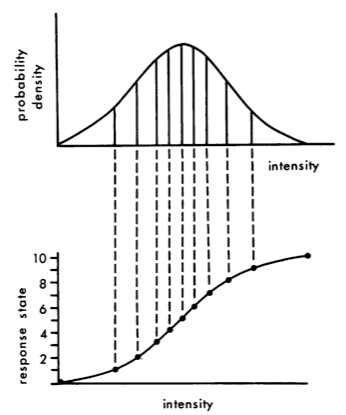
\includegraphics[width=0.5\textwidth]{laughlin1981-fig1}
	\label{fig:laughlin1981-fig1}
\end{figure}



% ---------------------------------------------------- %
%                    LAUGHLIN 1981                     %
% ---------------------------------------------------- %



% ---------------------------------------------------- %
%                     SIMONCELLI 2003                  %
% ---------------------------------------------------- %

\section{Vision and the Statistics of the Visual Environment}

% ---------------------------------------------------- %
%                     SIMONCELLI 2003                  %
% ---------------------------------------------------- %







% ---------------------------------------------------- %
%                 	REFERENCE LIST                     %
% ---------------------------------------------------- %

\begin{thebibliography}{99} 

\bibitem[Barlow 1961]{Barlow:1961dg}
Barlow, H.~B. (1961).
\newblock Possible Principles Underlying the Transformations of Sensory Messages.
\newblock {\em Sensory communication}, (1961):217-234.

\bibitem[Laughlin, 1981]{Laughlin:1981dg}
Laughlin, S. (1981).
\newblock A Simple Coding Procedure Enhances a Neuron's Information Capacity.
\newblock {\em Z. Naturforsch}, 36.910-912 (1981): 51.

\bibitem[Nirenberg et. al., 2001]{Nirenberg:2001dg}
Nirenberg, S., Carcieri, S.~M., Jacobs, A.~L., \& Latham, P.~E. (2001).
\newblock Retinal ganglion cells act largely as independent encoders.
\newblock {\em Nature}, 411(6838), 698-701.

\bibitem[Simoncelli 2003]{Simoncelli:2003dg}
Simoncelli, E.~P. (2003).
\newblock  Vision and the statistics of the visual environment.
\newblock {\em Current opinion in neurobiology}, 13(2), 144-149.
 
\end{thebibliography}

% ---------------------------------------------------- %
%                 	REFERENCE LIST                     %
% ---------------------------------------------------- %


\end{multicols}

\end{document}


% ---------------------------------------------------- %
